\documentclass[a4paper]{article}

\usepackage[utf8]{inputenc}
\usepackage{polski}
\usepackage{amsmath}
\usepackage{graphicx}
\usepackage[colorinlistoftodos]{todonotes}

\title{Dokumentacja użytkownika implementacji projektu nr 1. RW}

\author{Tomasz Półgrabia}

\date{\today}

\begin{document}
\maketitle

\begin{abstract}

\end{abstract}

\section{Wykorzystane technologie}
	Implementacja projektu nr 1. z RW będzie wykonana przy użyciu następujących technologii:
    \begin{itemize}
    	\item C\# (framework środowiska developerskiego .NET v4.5),
        \item prolog (implementacja SWI-prolog).
    \end{itemize}
    
    C\# zostanie wykorzystany w celu stworzenia wizualizacji zdarzeń zachodzących w czasie wykonania
    programu, natomiast prolog do implementacji logiki języka. Następnie zostanie wykorzystany
    interfejs C\# - prolog w celu zapewnienia komunikacji pomiędzy wyżej wymienionymi modułami.
    
    Do komunikacji pomiędzy modułami zostanie wykorzystana biblioteka SWIPlCs.
    
    \subsection{C\#}
    C\# to wielo paradygmatowy język programowania (głównie obiektowy)
    zaprojektowany przez zespół pod kierunkiem \textit{Andersa Hejlsberga}
    dla firmy \textit{Microsoft}. Program napisany w tym język kompilowane są
    do języka \textit{Common Intermediate Language} (\textit{CIL}),
    specjalnego kodu pośredniego wykonywanego w środowisku takim jak 
    \textit{.NET Framework}, open source \textit{Mono} czy \textit{DotGNU}.
    Wykonanie takiego kodu bez środowiska nie jest możliwe.

    Podstawowe cechy \textit{C\#} to:
    \begin{itemize}
        \item \textit{obiektowość} z hierarchią o jednym elemencie nadrzędnym,
        \item odśmiecanie pamięci (ang. garbage collector),
        \item właściwości, indeksery,
        \item delegaty, zdarzenia,
        \item typy ogólne,
        \item bogata biblioteka klas \textit{BCL}, umożliwiająca rozwijanie
            aplikacji konsolowych, okienkowych (\textit{Forms} czy \textit{WPF})
        \item ADO.NET,
    \end{itemize}

    C\# został wykorzystany głównie do stworzenia przyjaznego interfejsu
    dla użytkownika systemu.

    \subsection{Prolog}
    Prolog zostanie wykorzystany w projekcie \textit{TODO} w celu
    zaimplementowania logiki języka z domyślnymi akcjami. Prolog to
    jeden z popularniejszych języków programowania logicznego. Powstał on
    w celu automatycznej analizy języków naturalnych, jednakże jest on
    językiem ogólnego zastosowania i dobrze sprawdza się w programach 
    związanych ze sztuczną inteligencją. Program w Prologu składa się z faktów
    i reguł wnioskowania, aby go uruchomić należy wprowadzić odpowiednie 
    zapytanie. Prolog opiera się na rachunku predykatowym pierwszego rzędu,
    jednakże ogranicza się on do \textit{klauzul Horna}. Istnieją jednak
    wbudowane predykaty wyższego stopnia.

    \subsubsection{SWI-prolog}
        SWI-prolog to jedna z wielu otwarto-źródłowych implementacji prologa,
        ogólnie używana w celach edukacyjnych i sieci semantycznych. Ma bogaty
        zbiór cech i bibliotek wspierjących takie funkcjonalności jak:
        \begin{itemize}
            \item wielowątkowość,
            \item testowanie jednostkowe (ang. unit testing),
            \item GUI,
            \item interfejsy do Java, ODBC
            \item literate programming (pol. programowanie piśmienne),
            \item serwery web,
            \item SGML,
            \item RDF,
            \item RDFS,
            \item narzędzia developerskie (np. GUI debugger i GUI profiler),
            \item obszerną dokumentację.

        \end{itemize}

        Dzięki rozbudowanemu zbiorowi bibliotek, programowanie w prologu
        będzie łatwiejsze i wykluczy problemy w interfejsie c\# i prolog.

\section{Interfejs użytkownika}
    \subsection{Interfejs graficzny}

        Interfejs graficzny systemu \textit{AD} jest prosty w obsłudze.
        Składa się z jednego okna dialogowego z możliwością załadowania
        modelu z pliku ,,LOAD MODEL FILE'. Poniżej obu przycisków znajduje się pole tekstowe
        służące do wyrażenia zapytania (ang. query) w języku wejścia 
        systemu \textit{AD}.

        W załączniku są dołączone obrazy z działania aplikacji.

        \begin{figure}[p]
            \centering
            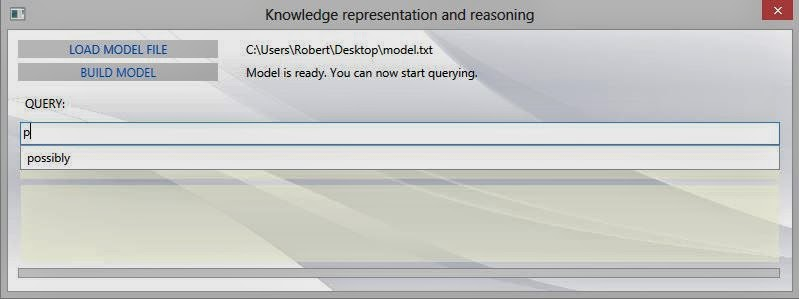
\includegraphics[width=\textwidth]{images/acomp_1.jpg}
            \caption{przykład auto - uzupełniania kwerendy nr 1}
            \label{fig:acomp1}
        \end{figure}

        \begin{figure}[p]
            \centering
            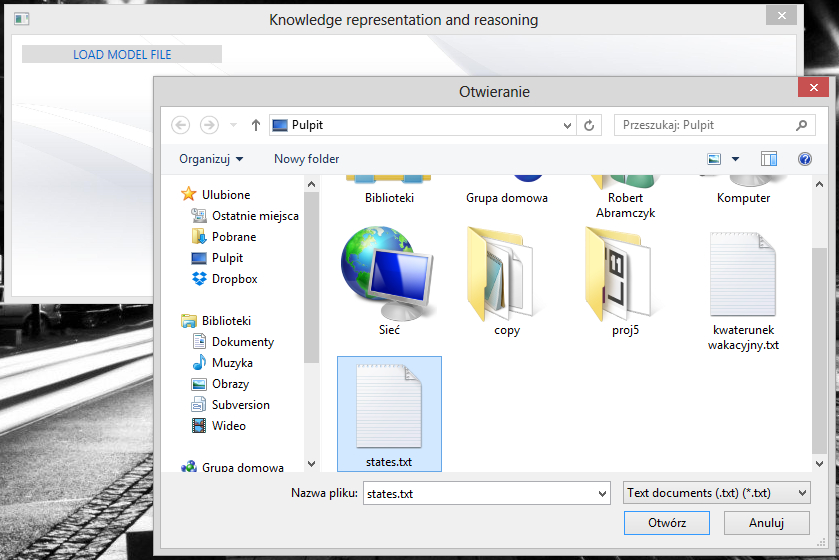
\includegraphics[width=\textwidth]{images/acomp_2.jpg}
            \caption{przykład auto - uzupełniania kwerendy nr 2}
            \label{fig:acomp2}
        \end{figure}

        \begin{figure}[p]
            \centering
            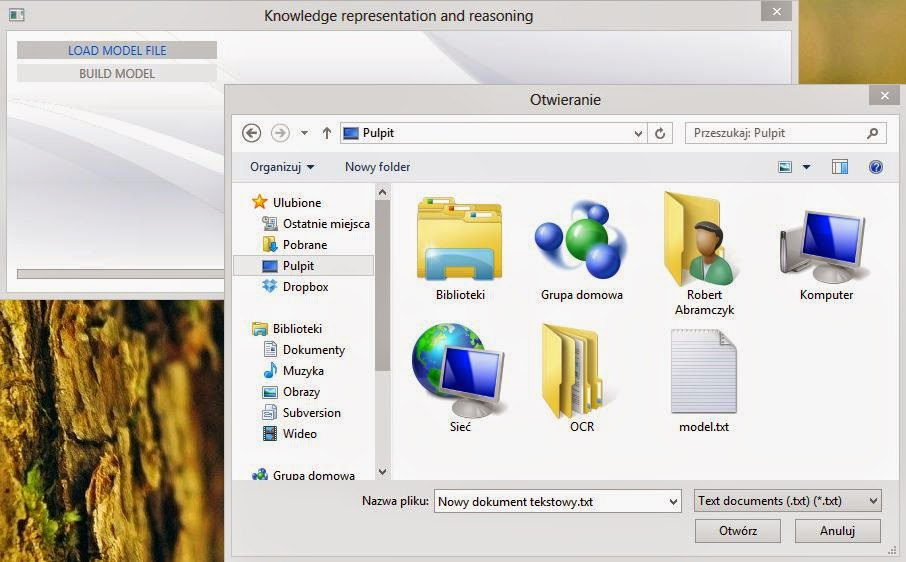
\includegraphics[width=\textwidth]{images/acomp_3.jpg}
            \caption{przykład ładowania modelu z pliku}
            \label{fig:acomp3}
        \end{figure}

    \subsection{Język modelu systemu}
        Język modelu dostarczanego do systemu przez klienta jest zgodny
        z językiem AD opisanego w specyfikacji języka \textit{AD} dostarczonej
        na laboratoria nr 1.

        Przykładowo:

        \begin{itemize}
            \item initially a - początkowo a jest prawdziwe,
            \item \textit{always $\gamma$ after $A_1, ... , A_n$ by 
                $E_1, ..., E_n$ from $\pi$} - po serii akcji wykonanych przez
                wykonawcą ze stanu $\pi$ zawsze prawdziwe jest $\gamma$.
        \end{itemize}

    \subsection{Język wejścia / kwerend}
        Język wejścia systemu \textit{AD} jest opisany w pełni w dokumencie 
        języka systemu \textit{AD}. Dane w takim języku są tłumaczone na kod
        wejścia prologu poprzez parser danych wejściowych.


    Przykładowo:
      
    \begin{itemize}
        \item \textit{ possibly executable $A_1, A_2, ..., A_n$ by $E_1, E_2, ... E_n$ from $\pi$ }
            zwróci użytkownikowi informacje o tym, czy ciąg akcji 
            $A_1, A_2, A_3, ..., A_N$ wykonanych przez ciąg wykonawców
            $E_1, E_2, ..., E_N$ jest możliwa do wykonania.
        \item \textit{ always executable  $A_1, A_2, ..., A_n$ by $E_1, E_2, ... E_n$ from $\pi$  }
            zwróci użytkownikowi informacje o tym, czy ciąg akcji
            $A_1, A_2, A_3, ..., A_N$ wykonanych przez ciąg wykonawców
            $E_1, E_2, ..., E_N$ jest zawsze możliwa do wykonania.

    \end{itemize}

\end{document}
